\chapter{Planification des trajectoires}


\section{Introduction}

Dans les précédents chapitre ont présentés des lois de commandes qui calculent les commandes à envoyer aux actionneurs pour obtenir soit des positions, des vitesses, des accélérations ou des forces désirée. Certaines loi de commandes nécessitait seulement une position finale cible alors que pour d'autre nous devions spécifier une position, une vitesse et une accélération en tout temps sur une trajectoire cible. Plusieurs tâches en robotique nécessite donc une couche intermédiaire entre des spécifications à haut niveau pour une tâche et les références qui doivent être fournit à une boucle de commande à bas niveau, cette étape intermédiaire est appelée la planification de trajectoire.

\video{Introduction à la planification de trajectoires}{https://youtu.be/_SQumKYdFnM}
%TODO: Refaire une introduction plus générique

\paragraph{Pourquoi donner directement la position finale désirée à un contrôleur bas niveau en position n'est pas toujours approprié?}
L'étape de planification de trajectoire est généralement essentiel lorsqu'un robot doit faire un mouvement de grande amplitude, i.e. lorsque la position cible est éloignée de la position actuelle. Les loi de commandes bas-niveau sont typiquement conçu pour garantir la convergence vers la position cible mais pas le détail du chemin pour s'y rendre ni la vitesse d'approche; plus la cible est loin, plus il va y avoir de raison de mieux contrôler les étapes intermédiaire pour ce rendre à la cible. Voici une liste non-exhaustive de raisons pour mieux contrôler le trajet jusqu'à une cible:
\begin{enumerate}
    \item \textbf{Obstacles et contraintes en position:} Parfois il y a des positions/configurations sur lesquelles on ne veux pas que le système robotique ce retrouve (collisions avec des obstacles, singularités, etc.). Les lois de commande simples vont typiquement allez directement droit vers la cible et possiblement la dépasser avant de se stabiliser sur celle-ci sans tenir compte de contraintes. Un planificateur de trajectoire peut déterminer un chemin à suivre pour atteindre la cible qui évite des obstacles et positions inadéquates.
    \item \textbf{Contraintes en vitesse:} Les contrôleurs simples vont typiquement tenter d'aller de plus en plus vite vers la cible proportionnellement avec l'erreur initiale sans tenir compte des limites physiques. Si des saturations à bas niveau font que la vitesse réelle ne suit pas la vitesse commandée le comportement et la convergence de la loi de commande sera incertain. De plus, pour des raisons de sécurité il peut être nécessaire de limiter la vitesse d'un robot. Un planificateur de trajectoire peut déterminer un profil de vitesse à suivre qui respecte des contraintes.
    \item \textbf{Faisabilité dynamique:} Finalement, surtout pour des robots dynamiques et/ou qui bougent rapidement, les lois de commande de base peuvent facilement se retrouver dans des situations ou ils demande des niveaux d'accélération ou de forces aux actionneurs qui se sont pas physiquement possible. Un planificateur peut permettre de déterminer une séquence d'action physiquement possible qui vont mener le robot jusqu'à la cible tout en respectant des contraintes.
\end{enumerate}

%TODO: Demo colab pendule swing-up avec et sans trajectoire cible



\section{Chemin et profil temporel}
\label{sec:chemin}

\note{Système de coordonnées pour définir une trajectoire}{On peut définir des trajectoires dans plusieurs systèmes de coordonnées. Toutefois, pour simplifier la notation, nous présenterons ici d'abord plusieurs concepts en considérant que le trajet est toujours définit dans l'espace des joints d'un robot. Nous verrons ensuite que ces concepts se généralisent pour d'autres systèmes de coordonnées. }

Il est parfois utile d'utiliser le concept d'un chemin pour découpler le problème de planification de trajectoire en deux étapes: 1) trouver un chemin, une description géométrique d'une séquence de configuration $\col{q}$ reliant le point de départ et la cible; et ensuite 2) déterminer un profil temporel de vitesse sur ce chemin pour fixer une trajectoire temporelle.

\begin{figure}[htbp]
	\centering
		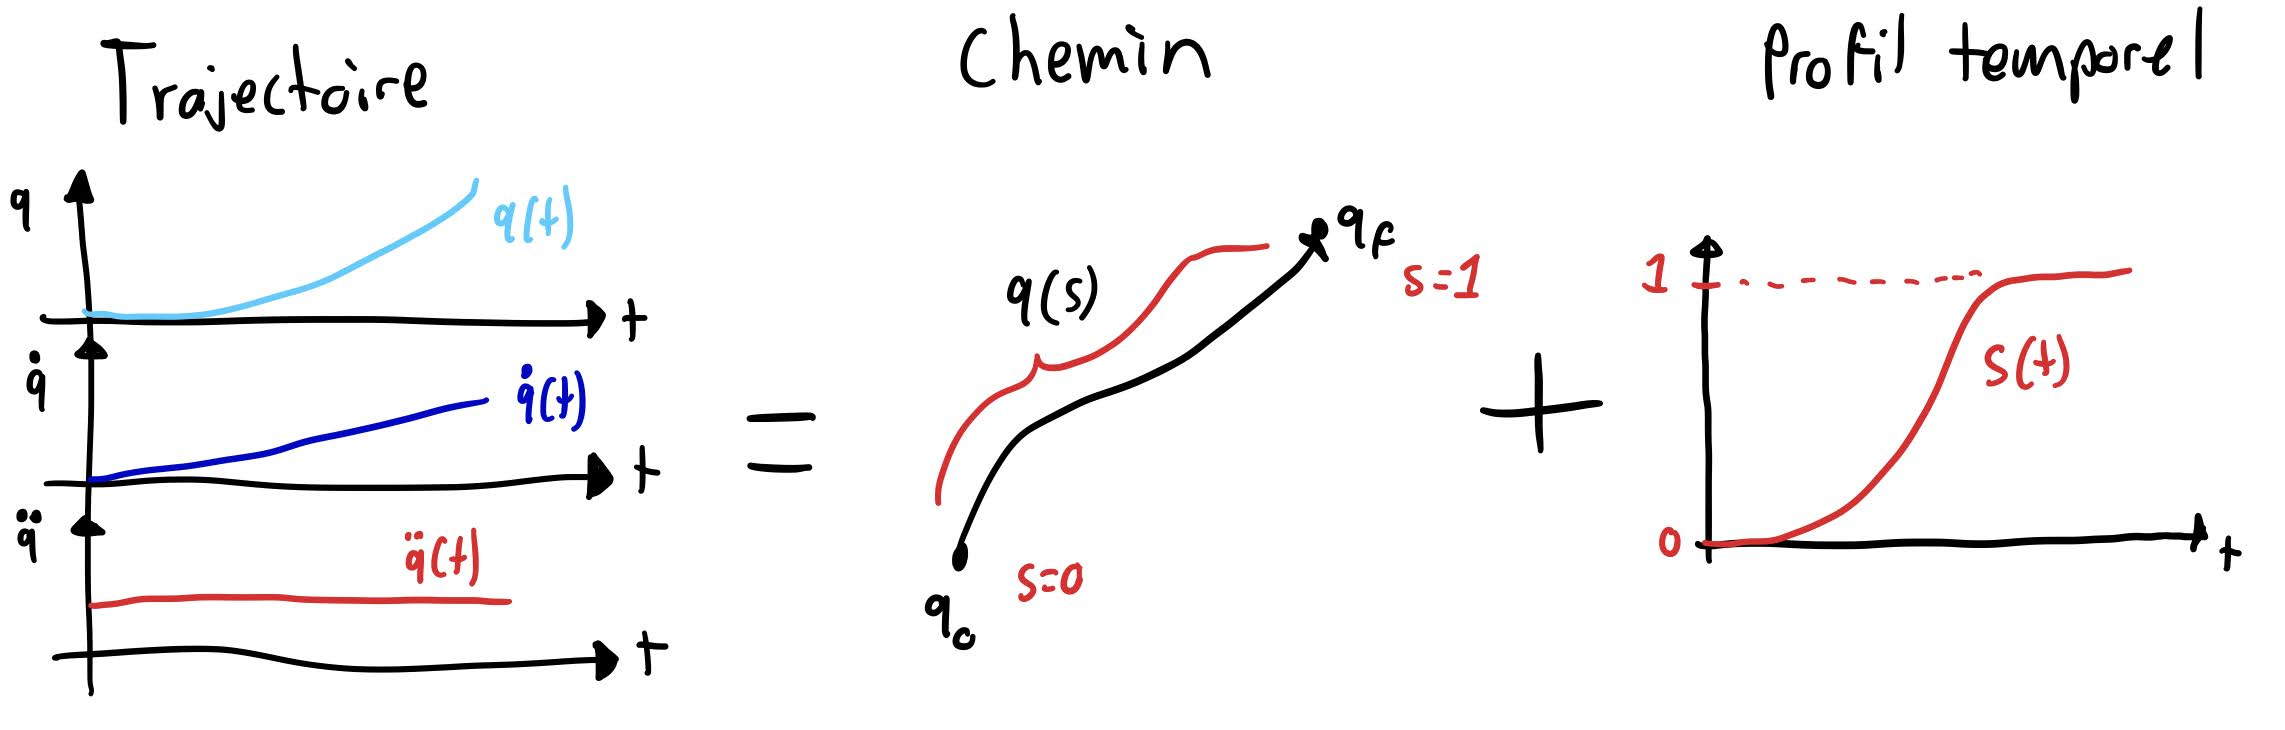
\includegraphics[width=0.90\textwidth]{fig/traj_path.jpg}
	\caption{Trajectoire (dans l'espace des joints), chemin et profil temporel}
	\label{fig:traj_path}
\end{figure}

\paragraph{Trajectoire} Une trajectoire est une fonction qui détermine la position d'un robot comme une fonction du temps $\col{q}(t)$. Normalement il est désirable d'avoir des fonctions qui sont dérivables deux fois, i.e. que la dérivé temporelle de cette fonction ne soit pas discontinue, ce qui impliquerait des accélérations d'amplitude infinie. La trajectoire est donc ultimement les trois fonctions suivantes:
\begin{align}
    \text{Trajectoire:} \quad \col{q}(t), \col{\dot{q}}(t), \col{\ddot{q}}(t) \quad \text{avec} \quad t \in [t_0,t_f]
\end{align}

\paragraph{Chemin} Une chemin est une fonction qui détermine la position d'un robot comme une fonction continue d'une variable scalaire $s \in [0,1]$, qui est égale à 0 au début du chemin et à 1 à la fin du chemin. 
\begin{align}
    \text{Chemin:} \quad \col{q}(s) \quad \text{avec} \quad s \in [0,1]
\end{align}

\paragraph{Profil temporel}  Un profil temporel est une trajectoire pour une variable scalaire intermédiaire qui caractérise la progression du système sur un chemin:
\begin{align}
    \text{Profil temporel:} \quad s(t), \dot{s}(t), \ddot{s}(t) \quad \text{avec} \quad t \in [t_0,t_f]
\end{align}

Lorsqu'on construit une fonction de trajectoire basé sur un chemin et un profil temporel on obtient les relations suivantes en appliquant une dérivée en chaîne :
\begin{align}
    \col{q}(t)       &=  \col{q}(s(t))\\
    \col{\dot{q}}(t) &= \frac{\partial \col{q}}{ \partial s}  \dot{s}    \\
    \col{\ddot{q}}(t)&= \frac{\partial \col{q}}{ \partial s}  \ddot{s} + \frac{\partial^2 \col{q}}{ \partial s^2}  \dot{s}^2
\end{align}


\subsection{Profils temporels}

Cette section présente quelques fonction de profil temporel qui sont typiquement utilisée pour générer des trajectoires.

\subsubsection{Profil temporel trapézoïdal}

Une profil de type trapézoïdal, voir Figure \ref{fig:trap_profile_speed}, est utilisé fréquemment comme base de génération de trajectoire simple pour plusieurs type de système asservis en position. Ce profil permet d'inclure directement une limite en vitesse $v_{max}$ et une limite en accélération $a_{max}$, c'est le profile qui donne la trajectoire la plus rapide possible considérant ces deux contraintes. Il existe toutefois des profils temporels plus lisses sans discontinuités, voir les prochaines sections, ce qui peut être un avantage. Le profile trapézoïdal consiste en trois phases: une phase d'accélération avec $\ddot{s} = a_{max}$, une phase de croisière a vitesse constante avec $\dot{s} = v_{max}$ et une phase de décélération avec $\ddot{s} = -a_{max}$. Les profils de positions et d'accélérations associés sont illustrés à la Figure \ref{fig:trap_profile_speed_all}.
\begin{figure}[htbp]
	\centering
		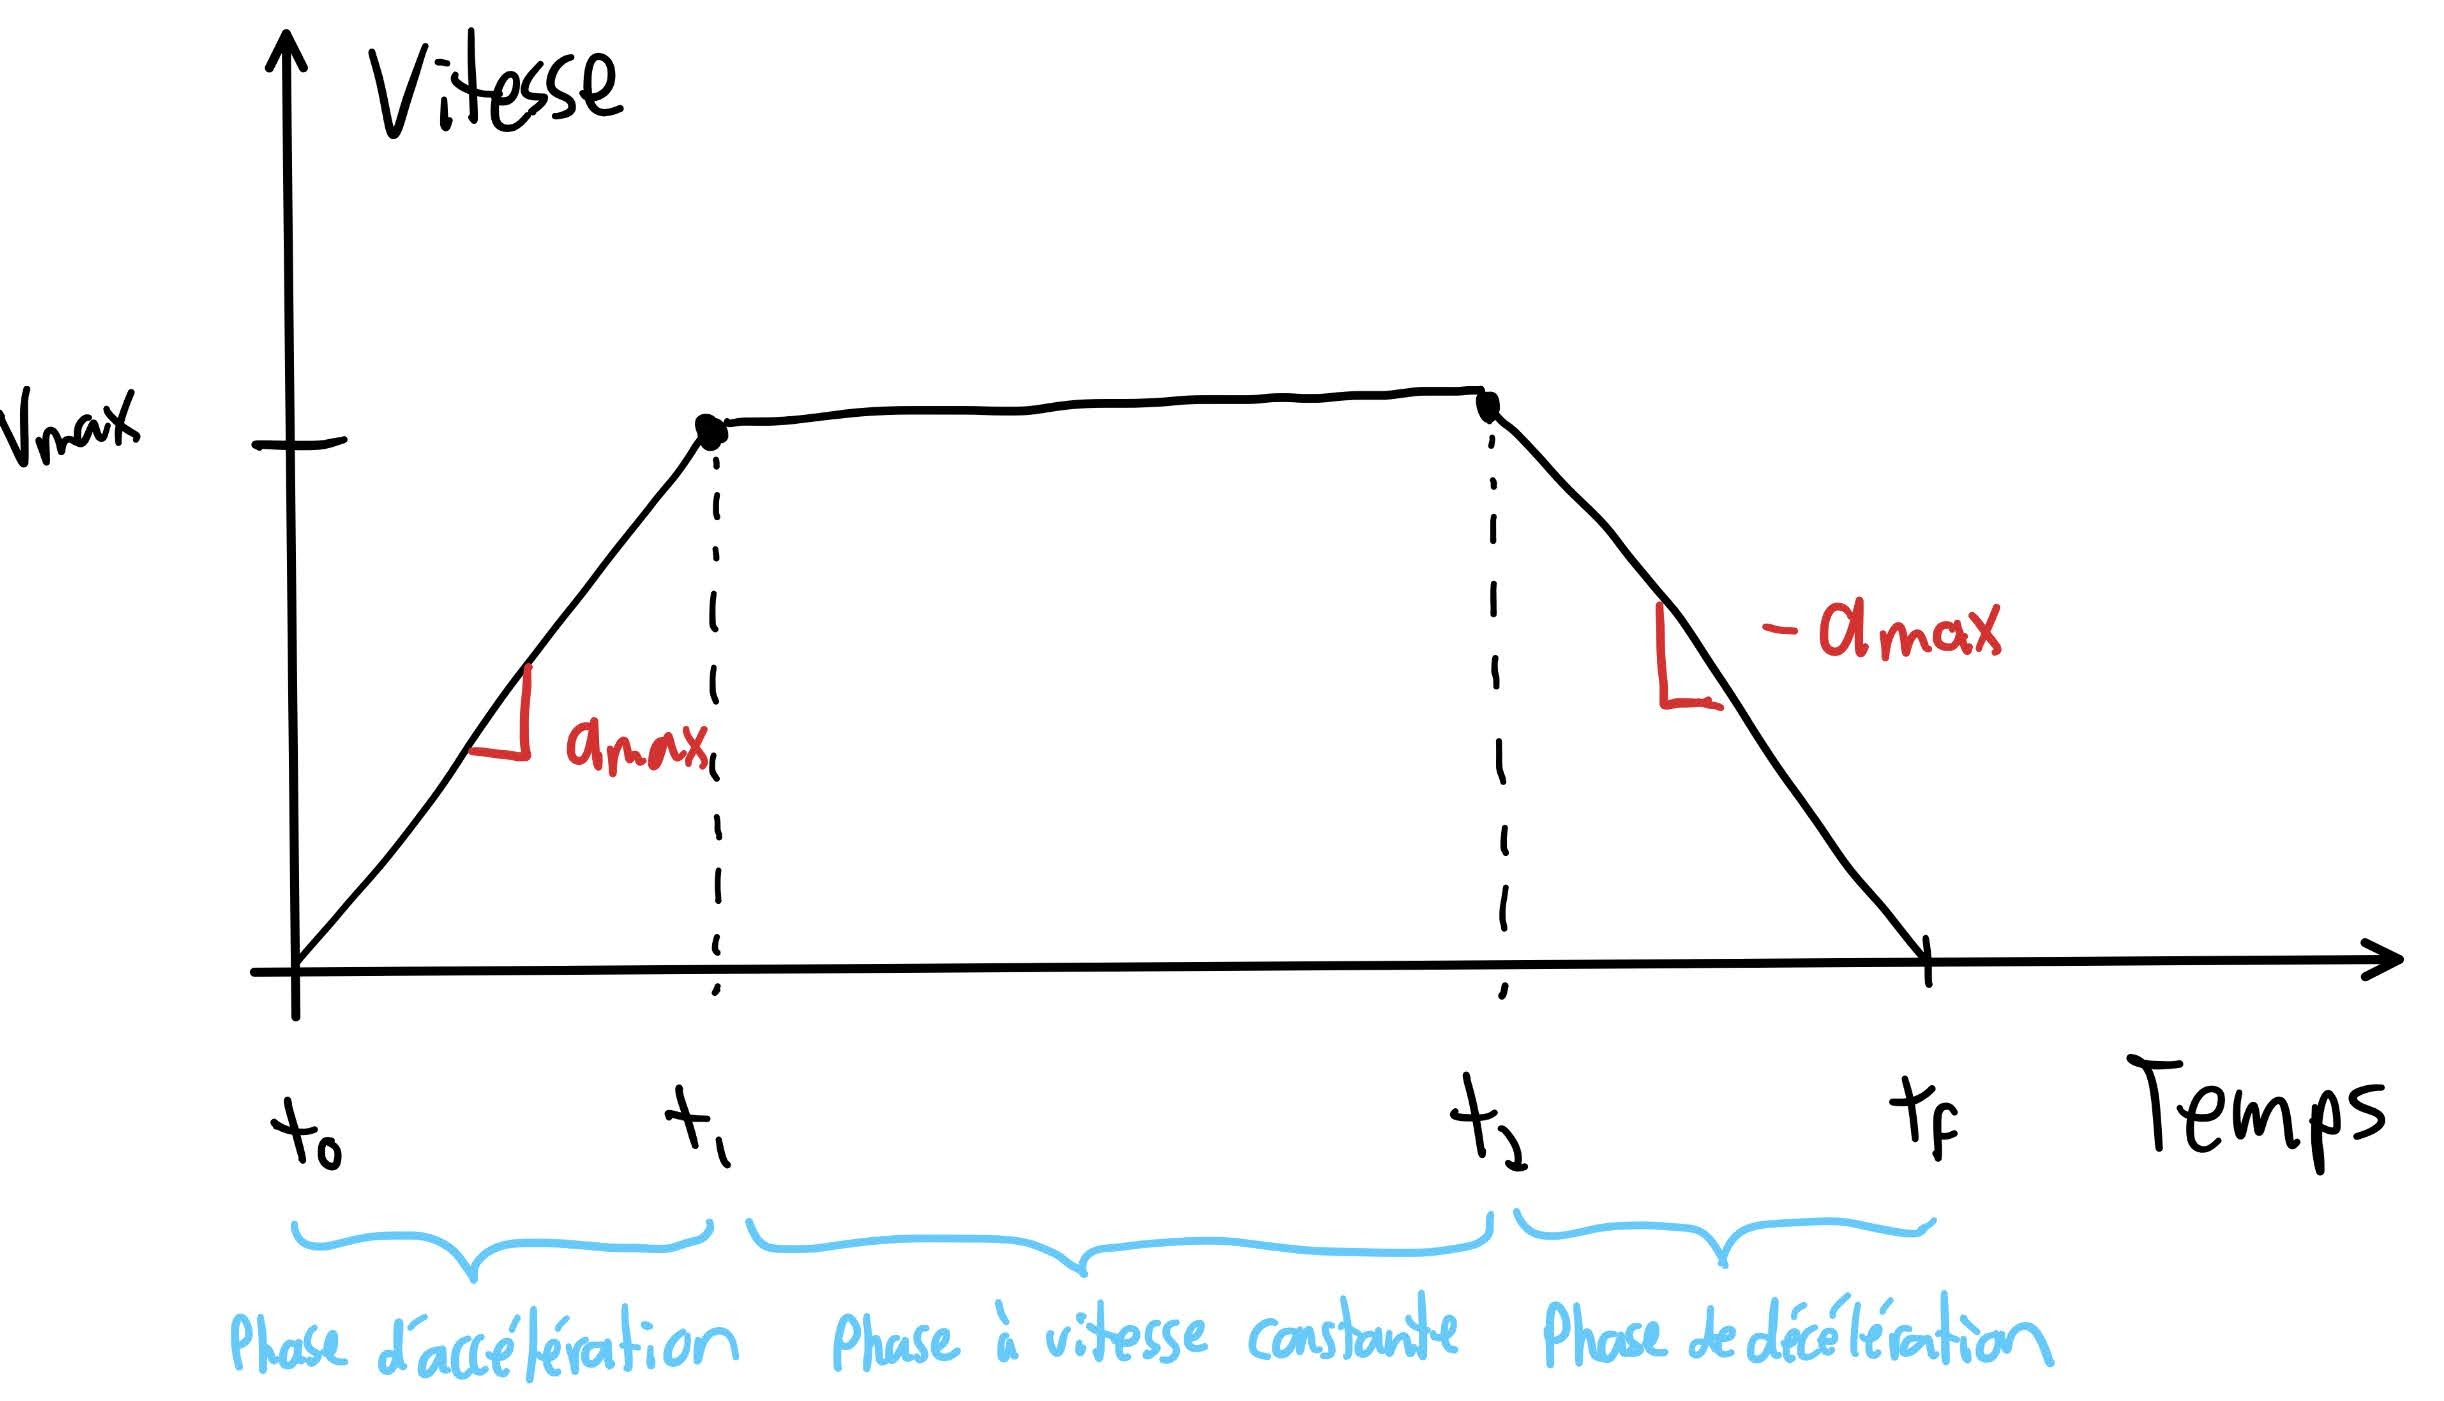
\includegraphics[width=0.70\textwidth]{fig/trap_profile_speed.jpg}
	\caption{Profil temporel de vitesse de type trapézoïdal}
	\label{fig:trap_profile_speed}
\end{figure}

\begin{figure}[htbp]
	\centering
		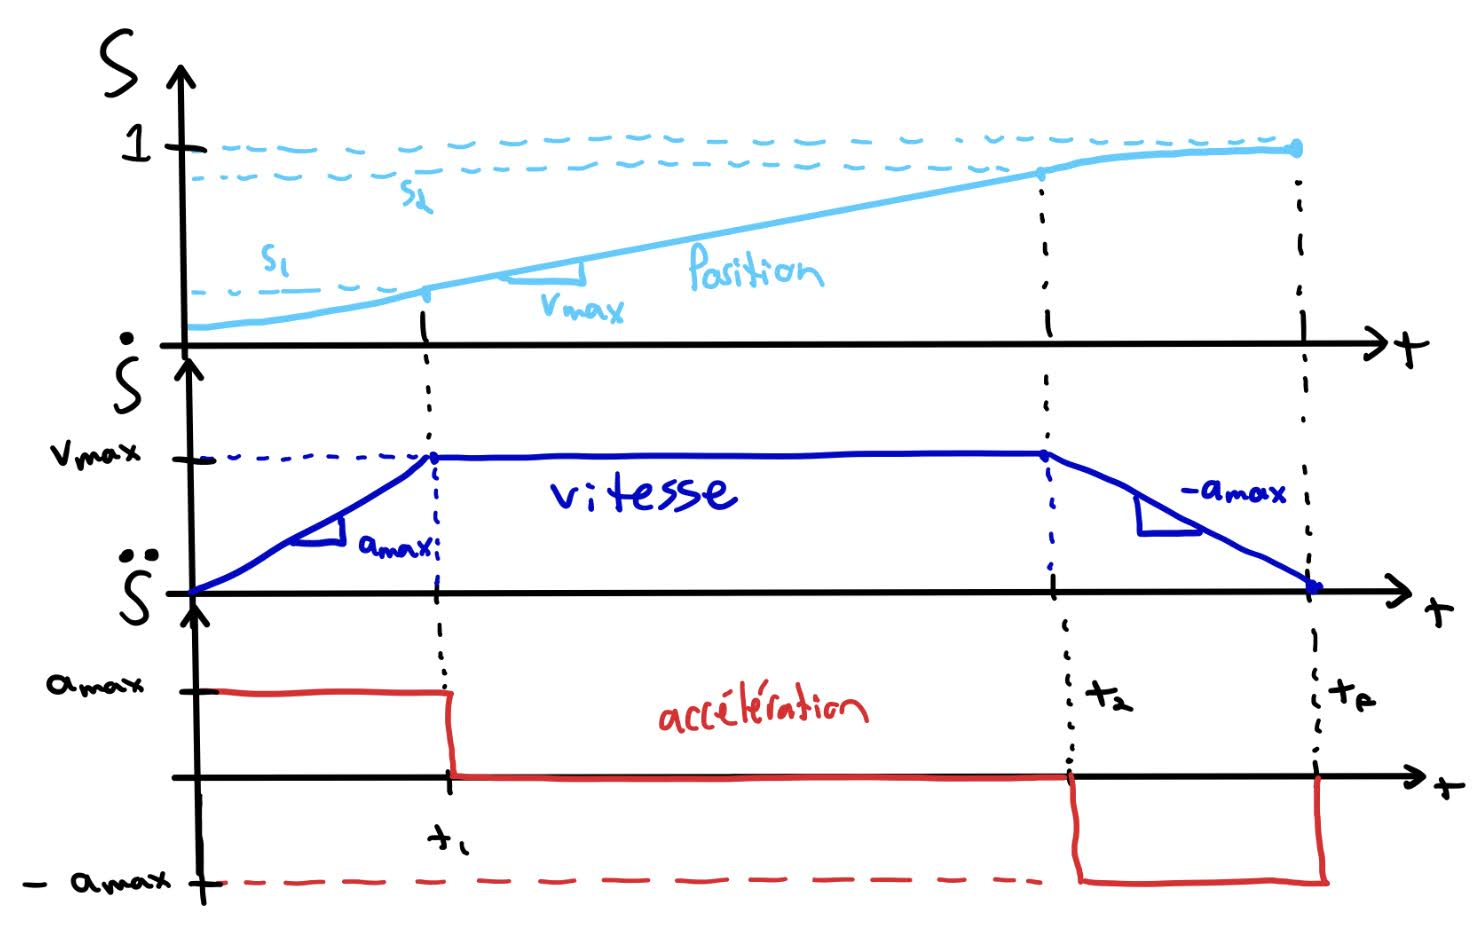
\includegraphics[width=0.70\textwidth]{fig/trap_profile_all.jpg}
	\caption{Position, vitesse et accélération pour un profil temporel de type trapézoïdal}
	\label{fig:trap_profile_speed_all}
\end{figure}

Un profile trapézoïdal peut être définit à partir de 4 variables: la vitesse maximale $v_{max}$, l'accélération maximale $a_{max}$, la durée totale $T=t_f-t_0$ et le déplacement total $s_f$, parmi lesquels seulement deux sont indépendantes. Si on utilise le profil pour ajuster le temps sur un chemin prédéfini (voir section \ref{sec:chemin}, le déplacement total est déjà fixé $s_f=1$ et on peut choisir deux variables à fixer parmi $T$, $v_{max}$ et $a_{max}$. Ensuite, si $\frac{v_{max}^2}{a_{max}} > 1$ le système n'a pas le temps d'atteindre sa vitesse maximale de croisière et le profil est réduite à deux phase: accélération et décélération, voir Figure XXX.

Lorsque $\frac{v_{max}^2}{a_{max}} \leq 1$, les équations de ce profile pour les trois segments temporels sont:
%%%%%%%%%%%%%%%%%%
\begin{align}
\text{si} \quad 0 \leq t \leq \frac{v_{max}}{a_{max}} \quad & \quad \left\{ \begin{array}{l}
s(t)= \frac{1}{2} a_{max} t^2
\\
\dot{s}(t)= a_{max} t
\\
\ddot{s}(t) = a_{max}
\end{array}
\right. \\
\text{si} \quad \frac{v_{max}}{a_{max}} < t \leq T- \frac{v_{max}}{a_{max}} \quad & \quad \left\{ \begin{array}{l}
s(t)= v_{max} t -  \frac{v_{max}^2}{2a}
\\
\dot{s}(t)= v_{max}
\\
\ddot{s}(t) = 0
\end{array}
\right. \\
\text{si} \quad  T- \frac{v_{max}}{a_{max}}  < t \leq T \quad & \quad \left\{ \begin{array}{l}
s(t) = \frac{2 a_{max} v_{max} T - 2 v_{max}^2 - a_{max}^2(t-T)^2}{2 a_{max}}
\\
\dot{s}(t)= a(T - t)
\\
\ddot{s}(t) = -a
\end{array}
\right.
\end{align}
%%%%%%%%%%%%%%%%%

\subsubsection{Profil temporel polynomial d'ordre 3}

\subsubsection{Profil temporel polynomial d'ordre 5}


\newpage
\section{Planification cinématique pour les robots manipulateurs}

\subsection{Ligne droite dans l'espace de la tâche}

\subsection{Ligne droite dans l'espace des joints}

Dans cette section, 

%
\begin{align}
  \ddot{\col{q}}_d(:),\dot{\col{q}}_d(:),\col{q}_d(:) = plan(\col{q}_{0}, \col{q}_f)
	\label{eq:trajgen}
\end{align}
%

ref p.163



\subsection{Point à point}
À venir!

\subsection{Multi-points}
À venir!



\subsection{Planification dans l'espace de la tâche}
À venir!



\section{Algorithmes d'optimisation de trajectoires}

\video{Introduction à la commande optimale}{https://youtu.be/3x6Vg-RRZ50}

\colab{Démo d'introduction à l'optimisation de trajectoires}{https://colab.research.google.com/drive/1yq2GHAkvO6fTF2W-tRbACDBa9_scec2k?usp=sharing}

À venir!

\section{Algorithmes de recherche}

À venir!
